  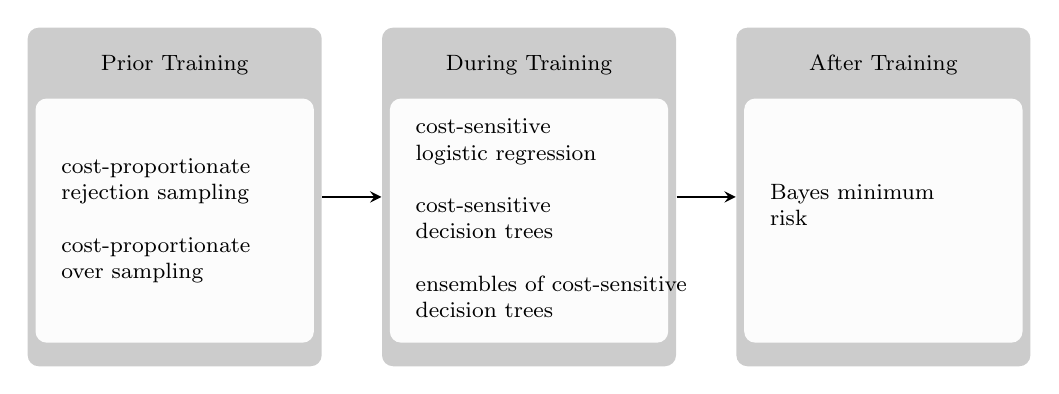
\begin{tikzpicture}[node distance=2.5cm]
  \tikzstyle{every node}=[font=\footnotesize]
  
  % Main boxes
  \node (data1) [rectangle, rounded corners, minimum width=2cm, minimum height=4.3cm,text 
                centered, fill=black!20, text width=3.5cm] 
                {\tabular{c} Prior Training\\ \\ \\ \\ \\ \\ \\ \\ \\ \\ \\ \endtabular};
  \node (data2) [rectangle, rounded corners, minimum width=2cm, minimum height=4.3cm,text 
                centered, fill=black!20, right of=data1, xshift=2cm, text width=3.5cm] 
                {\tabular{c} During Training\\ \\ \\ \\ \\ \\ \\ \\ \\ \\ \\ \endtabular};
  \node (data3) [rectangle, rounded corners, minimum width=2cm, minimum height=4.3cm,text 
                centered, fill=black!20, right of=data2, xshift=2cm, text width=3.5cm] 
                {\tabular{c} After Training\\ \\ \\ \\ \\ \\ \\ \\ \\ \\ \\  \endtabular};

  \node (data11) [rectangle, rounded corners, minimum width=2cm, minimum height=3.1cm, 
                fill=black!1, below of=data1, yshift=2.2cm, text width=3.3cm]
                {\tabular{l} cost-proportionate \\ rejection sampling \\ \\ cost-proportionate \\ 
                over sampling\\ \endtabular};

  \node (data21) [rectangle, rounded corners, minimum width=2cm, minimum height=3.1cm, 
                fill=black!1, below of=data2, yshift=2.2cm, text width=3.3cm]
                {\tabular{l}  cost-sensitive \\ logistic regression \\ \\ cost-sensitive \\ decision 
trees \\ \\ ensembles of cost-sensitive \\ decision trees \endtabular};
  
  \node (data31) [rectangle, rounded corners, minimum width=2cm, minimum height=3.1cm, 
                fill=black!1, below of=data3, yshift=2.2cm, text width=3.3cm]
                {\tabular{l}  \\ Bayes minimum\\ risk \\ \\  \\ \endtabular};
	
	% Arrows
	\draw[thick,->,>=stealth] (data1) to (data2);
  \draw[thick,->,>=stealth] (data2) to (data3);
  \end{tikzpicture}
 
%  \tikzstyle{startstop} = [rectangle, rounded corners, minimum width=2cm, minimum height=4cm,text 
% centered, draw=black, fill=black!20]
% \tikzstyle{startstop2} = [rectangle, rounded corners, minimum width=2cm, minimum height=1cm,text 
% centered, draw=black, fill=black!20]
% \tikzstyle{startstop3} = [rectangle, rounded corners, minimum width=2cm, minimum height=2.9cm,text 
% left, draw=black, fill=black!1]
% \tikzstyle{arrow} = [thick,->,>=stealth]